\textbf{\section{Tahapan Penelitian}}

% TODO: lengkapi
\begin{subs}
	\subsection{Pengumpulan Data}
	\indent

	Tahapan pengumpulan data dalam penelitian ini dilakukan untuk mendapatkan data historis pergerakan harga saham pada indeks LQ45 yang akan digunakan sebagai basis analisis prediksi. Proses pengumpulan data dilakukan dengan langkah-langkah sebagai berikut:
	\begin{enumerate}
		\item Pemilihan Emiten \\
		      Data yang dikumpulkan hanya mencakup saham-saham dari perusahaan yang masuk dalam indeks LQ45 pada periode tertentu. Emiten-emiten ini dipilih karena mereka mewakili perusahaan-perusahaan yang memiliki likuiditas tinggi dan stabilitas keuangan yang relatif baik.

		\item Jenis Data yang Dikumpulkan \\
		      Data historis yang dikumpulkan meliputi:
		      \begin{itemize}
			      \item Harga pembukaan (opening price)
			      \item Harga penutupan (closing price)
			      \item Harga tertinggi (high price)
			      \item Harga terendah (low price)
			      \item Volume perdagangan (trading volume)
		      \end{itemize}

		\item Platform Pengumpulan Data \\
		      Data diperoleh melalui fitur pengunduhan yang disediakan oleh Yahoo Finance. Platform ini dipilih karena:
		      \begin{itemize}
			      \item Menyediakan data historis secara gratis dan mudah diakses.
			      \item Format data yang dapat diunduh (seperti CSV) memudahkan proses analisis lebih lanjut.
		      \end{itemize}

		\item Proses Pengambilan Data \\
		      \renewcommand{\labelenumi}{\alph{enumi}.}
		      \begin{enumerate}
			      \item Melihat data yang tersedia pada \href{https://finance.yahoo.com}{Yahoo Finance}
			      \item Memasukkan kode saham dari emiten yang terdaftar dalam indeks LQ45.
			      \item Menginstall python untuk melakukan analisis serta pengambilan data.
			      \item Menginstall library yfinance untuk melakukan pengambilan data.
			      \item Menulis kode python untuk mengunduh dataset dari yahoo finance dengan memasukkan kode saham sesuai kode pada saham LQ45.
		      \end{enumerate}

		\item Validasi dan Verifikasi Data \\
		      Setelah data dikumpulkan, dilakukan proses validasi untuk memastikan data yang diperoleh sesuai dengan kebutuhan penelitian. Langkah-langkah validasi meliputi:
		      \begin{itemize}
			      \item Memeriksa konsistensi data (tidak ada duplikasi atau nilai yang hilang).
			      \item Memastikan kelengkapan data untuk setiap emiten yang dipilih.
			      \item Menyelaraskan format data agar kompatibel dengan alat analisis, seperti Python dan Pandas.
		      \end{itemize}


	\end{enumerate}

	\subsection{Preprocessing Data}
	\renewcommand{\labelenumi}{\alph{enumi}.}
	\indent

	Preprocessing data adalah tahap untuk membersihkan, mengubah, dan mempersiapkan data agar sesuai untuk digunakan dalam model machine learning. Langkah ini penting untuk memastikan data yang digunakan bersih, relevan, dan terstruktur.
	\begin{enumerate}
		\item Cleaning Data
		      Cleaning data atau pembersihan data merupakan sebuah proses yang sangat penting dalam penelitian untuk memisahkan data yang kotor seperti data yang hilang dan juga menghapus data kolom yang tidak relevan.
		\item Normalization Data
		      Normalization data adalah proses untuk mengatur data yang bervariasi antara satu sama lain menjadi data yang relatif yang sama. Proses ini dapat dilakukan dengan menggunakan metode-metode yang berbeda seperti min-max scaling, z-score, dan standarisasi. Data akan diubah ke dalam rentang 0 hingga 1 menggunakan metode MinMaxScaler untuk meningkatkan efisiensi model
		      \begin{lstlisting}
            import numpy as np
            from sklearn.preprocessing import MinMaxScaler

            data = np.array([1, 2, 3, 4, 5])
            scaler = MinMaxScaler()
            normalized_data = scaler.fit_transform(data.reshape(-1, 1))
            print(normalized_data)
        \end{lstlisting}
		\item Feature Engineering
		      Membuat fungsi untuk membagi data menjadi sekumpulan urutan waktu (sequences) dan label
		      \begin{lstlisting}
            def create_dataset(dataset, sequence_length=50):
            x, y = [], []
            for i in range(len(dataset) - sequence_length):
            x.append(dataset[i:i + sequence_length])
            y.append(dataset[i + sequence_length])
            return np.array(x), np.array(y)

            x, y = create_dataset(normalized_data)
          \end{lstlisting}
	\end{enumerate}

	\subsection{Pembagian Dataset}
	\indent

	Dalam penelitian ini, dataset akan dibagi menjadi dua set data yaitu, training data dan testing data. Training data digunakan untuk membuat model dan testing data digunakan untuk mengevaluasi model yang telah dibuat.
	Dalam penelitian ini data yang digunakan untuk proses latihan sebesar 80\% dan untuk validasi sebesar 20\%.
	\begin{lstlisting}
    train_size = int(len(x) * 0.8)
    x_train, x_test = x[:train_size], x[train_size:]
    y_train, y_test = y[:train_size], y[train_size:]
  \end{lstlisting}

	\subsection{Pemilihan Model}
	\indent

	Pemilihan model dan pelatihan bertujuan untuk memilih algoritma yang sesuai dengan kebutuhan penelitian. Pelatihan model dilakukan dengan memberikan data latih sehingga model dapat belajar pola dari data tersebut.
	Di Penelitian ini, model yang akan digunakan adalah LSTM. dikarenakan LSTM memiliki kemampuan untuk menganalisis data urutan waktu dan memprediksi data masa depan yang jauh lebih akurat dibanding dengan model tradisional seperti ARIMA dan model-model lainnya.

	\subsection{Evaluasi Model}
	\indent

	Evaluasi model adalah proses untuk mengukur kinerja model yang telah dilatih menggunakan metrik tertentu. Dalam penelitian ini, evaluasi dilakukan dengan membandingkan hasil prediksi dengan data aktual menggunakan Loss Function, Mean Squared Error (MSE) dan Mean Absolute Error (MAE).
	\begin{itemize}
		\item Mean Squared Error (MSE)
		      MSE adalah salah satu metrik yang paling umum digunakan untuk mengevaluasi model regresi, termasuk model LSTM. Metrik ini menghitung rata-rata dari kuadrat selisih antara nilai yang diprediksi dan nilai yang sebenarnya. MSE lebih sensitif terhadap kesalahan yang lebih besar karena setiap kesalahan dipangkatkan dua kali, sehingga kesalahan besar akan memberikan dampak yang lebih besar pada hasilnya.
		\item Mean Absolute Error (MAE)
		      MAE adalah metrik yang menghitung rata-rata dari nilai absolut perbedaan antara nilai yang diprediksi dan nilai yang sebenarnya. Berbeda dengan MSE, MAE tidak memberikan penalti yang lebih besar pada kesalahan besar, sehingga lebih robust terhadap outlier.
		\item Loss Function
		      Loss function adalah fungsi yang digunakan oleh model selama proses pelatihan untuk mengukur seberapa baik atau buruk prediksi model dibandingkan dengan nilai yang sebenarnya. Loss function bertujuan untuk mengoptimalkan kinerja model dengan meminimalkan nilai loss function selama pelatihan.

		      Pada model LSTM, loss function yang sering digunakan adalah Mean Squared Error (MSE), tetapi bisa juga menggunakan Mean Absolute Error (MAE) atau jenis loss function lainnya tergantung pada jenis model dan masalah yang dihadapi. Selama pelatihan, model LSTM mencoba meminimalkan nilai loss function melalui algoritma optimasi seperti Adam, SGD, atau lainnya.
	\end{itemize}

	\subsection{Analisis Hasil \& Visualisasi}
	Tahap ini bertujuan untuk memahami hasil yang diperoleh dari model dan menyajikannya dalam bentuk yang mudah dipahami, seperti grafik atau tabel.
	\begin{figure}[H]
		\centering
		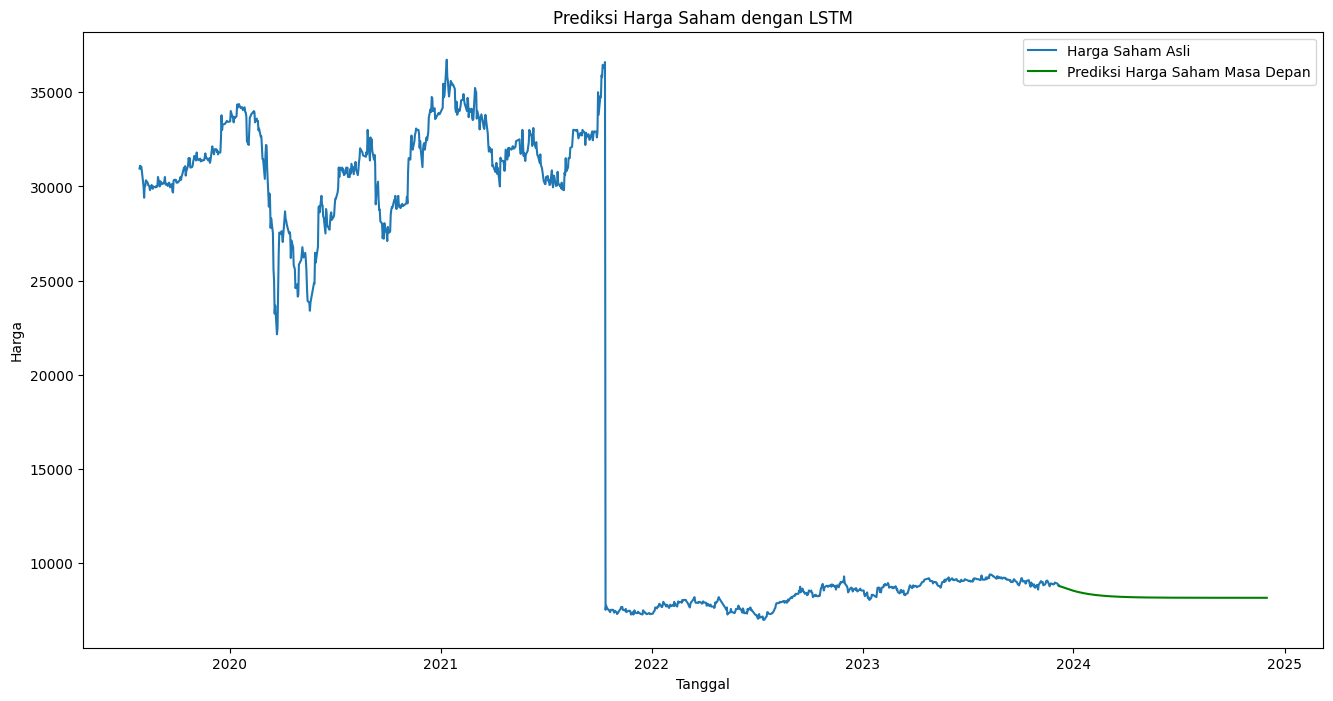
\includegraphics[width=0.8\textwidth]{hasil_analisis.png}
		\caption{Grafik hasil analisis}
	\end{figure}


\end{subs}
